\documentclass[10pt, aspectratio=169, compress]{beamer}
\usetheme[progressbar=frame title, numbering=fraction]{metropolis}      % Use metropolis theme 
\setbeamertemplate{section in toc}[sections numbered]
\setbeamertemplate{subsection in toc}[subsections numbered]
\useoutertheme[subsection=false]{miniframes}
\setbeamercolor{section in head/foot}{fg=white, bg=mDarkTeal}
\setbeamercolor{background canvas}{bg=white}
\setbeamerfont{section in head/foot}{series=\bfseries}

\usefonttheme[onlymath]{serif}
\usepackage{amsmath}
\usepackage{remreset}
\usepackage{ragged2e}
\usepackage{booktabs}
\usepackage{makecell}
\usepackage{float}
\usepackage{subfig}
\usepackage{tikz}
\usetikzlibrary{positioning,calc,trees}
\usepackage[flushleft]{threeparttable}	% 3 part table 
\usepackage[justification=centering]{caption}
\captionsetup{skip=0pt}
\graphicspath{{./fig/}}

\makeatletter
\let\beamer@writeslidentry@miniframeson=\beamer@writeslidentry
\def\beamer@writeslidentry@miniframesoff{%
	\expandafter\beamer@ifempty\expandafter{\beamer@framestartpage}{}% does not happen normally
	{%else
		% removed \addtocontents commands
		\clearpage\beamer@notesactions%
	}
}
\newcommand*{\miniframeson}{\let\beamer@writeslidentry=\beamer@writeslidentry@miniframeson}
\newcommand*{\miniframesoff}{\let\beamer@writeslidentry=\beamer@writeslidentry@miniframesoff}
\beamer@compresstrue
\makeatother

%==============================================================
% Title Page
%==============================================================
%Information to be included in the title page:
\title{Exportando tablas en Stata I}
\subtitle{Replicación de Papers\\Basado en ``Nice and fast tables in Stata'' del Banco Mundial}
\author{Rony Rodriguez-Ramírez} 
\institute{LAMBDA}
\titlegraphic{\hfill
\includegraphics[height=1.5cm]{dime}}
\date{\today}
%==============================================================
\begin{document}
%------------------------------------------------	
\begin{frame}[plain]
	\maketitle 
\end{frame}
%------------------------------------------------
\section{Introducción}
%-----------------------------------------------
\subsection{Introducción}
%-----------------------------------------------
\begin{frame}[t]{Inputs}
	\begin{itemize}
		\item Al incorporar tablas en documentos, es común copiar y pegar resultados y formatearlos en Word.
		\item En nuestra experiencia, esta práctica es a menudo una restricción a la reproducibilidad.
	\end{itemize}
\end{frame}
%------------------------------------------------
\section{Dos etapas para programar tablas}
%-----------------------------------------------
\subsection{Dos etapas para programar tablas}
%-----------------------------------------------
\begin{frame}[t]
	\frametitle{Antes de implementar el código, pregúntate}

	\begin{itemize}[<+->]
		\item ¿Necesito que esta salida se pueda compartir inmediatamente sin procesamiento posterior?
		\item ¿Esta salida está lista para su publicación, o solo para descubrimiento y exploración?
		\item ¿Necesito poder ajustar el formato y redondeo de números más tarde?
		\item ¿Tendré que ajustar el diseño y el formato de la tabla más adelante?
		\item ¿Cuál será el flujo de trabajo requerido cuando vuelva a producir esta tabla?
		\item ¿Qué pasará con la tabla si modifico modelos, parámetros u otros componentes centrales?
		\item ¿Es probable que altere los modelos, parámetros u otros componentes principales?
	\end{itemize}
\end{frame}
%-----------------------------------------------
\begin{frame}
	\frametitle{Dos procesos}

	\begin{columns}
		\begin{column}[t]{0.5\textwidth}
			\textbf{Stage 1:} 
			\begin{itemize}
				\item Tablas mínimamente formateadas y anotadas
				\item El diseño de la tabla se ajustará repetidamente
				\item No pierdas mucho tiempo haciendo que tus mesas se vean súper bonitas en esta etapa
			\end{itemize}
		\end{column}
		\begin{column}[t]{0.5\textwidth}  %%<--- here
			\textbf{Stage 2:} 
			\begin{itemize}
				\item Compartir tablas fáciles de leer con investigadores o formuladores de políticas.
				\item Salida reproducible y con buen formato, lista para su publicación.
				\item El equipo ha acordado el conjunto básico de resultados y cómo presentarlos.
			\end{itemize}
		\end{column}
	\end{columns}

\end{frame}
%-----------------------------------------------
\begin{frame}
	\frametitle{Eligiendo software}

	\begin{columns}[t]
		\begin{column}{00.5\textwidth}
			\textbf{Excel:} 

			Ampliamente adoptado y accesible.
			El formateo es un proceso en gran parte manual, que ralentiza las ejecuciones de replicación.
		\end{column}
		\begin{column}{00.5\textwidth}
			\textbf{\LaTeX:}

			Tablas de actualización automática en informes y presentaciones. Costo fijo en el aprendizaje del lenguaje de formateo.
		\end{column}	
	\end{columns}

\end{frame}
%-----------------------------------------------
\begin{frame}
	\frametitle{Esquema}

	\begin{enumerate}
		\item Flujo de trabajo para la creación de tablas
		\item Opciones de softwares
		\item \texttt{esttab} demo
	\end{enumerate}	

\end{frame}
%==============================================================
\miniframesoff 	

\begin{frame}[plain, noframenumbering]
	\begin{center}
	\LARGE STATA TIME
		\begin{figure}[H]
			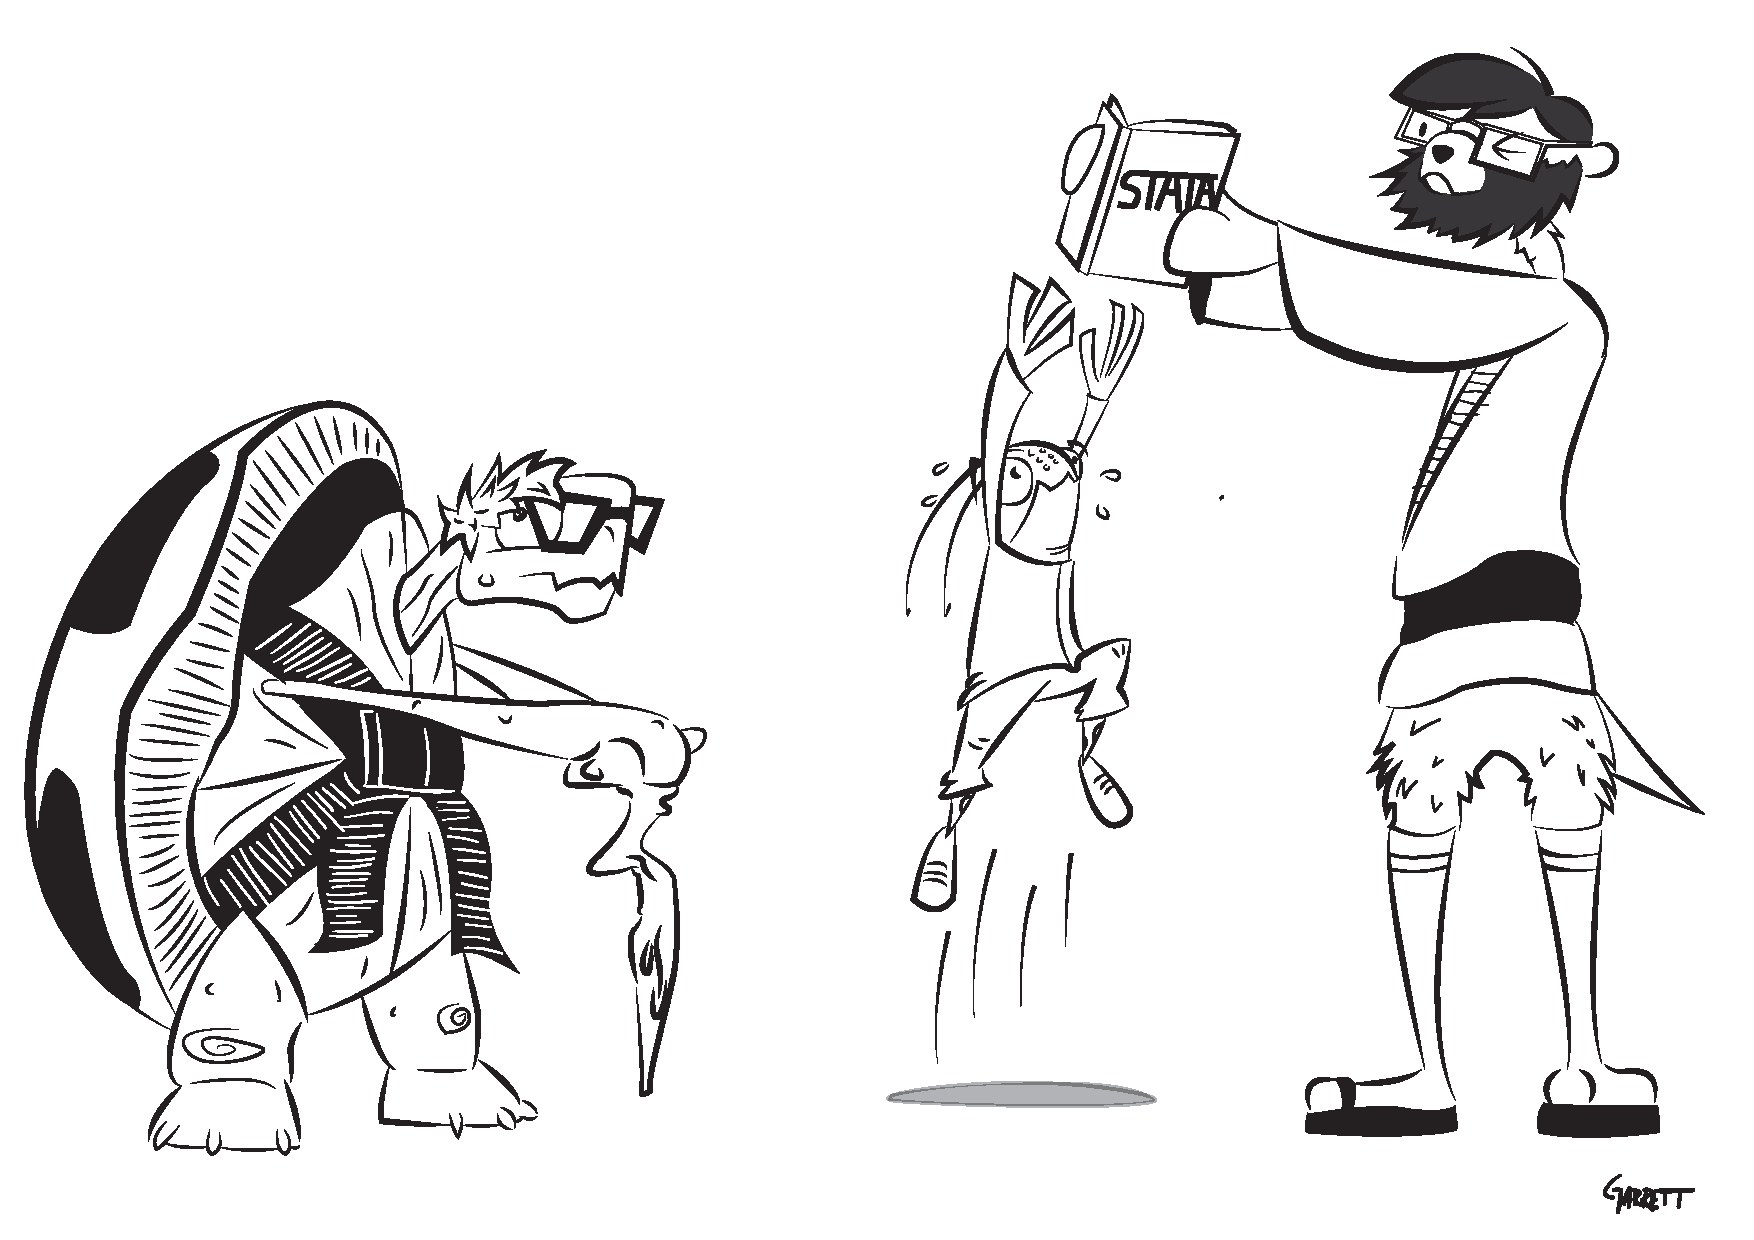
\includegraphics[width=0.57\textwidth]{stata.pdf}
		\end{figure}
	\end{center}
\end{frame}
%==============================================================
% END
%==============================================================	
\begin{frame}[plain, standout]
	Nos vemos mañana.
\end{frame}
%-----------------------------------------------
\end{document}		
